% chapters/glitch.tex
%
% Copyright 2023 Alexander Lyttle.
%
% This work may be distributed and/or modified under the conditions of the
% LaTeX Project Public License (LPPL) version 1.3 or later.
%
% The latest version of this license is in
% https://www.latex-project.org/lppl.txt and version 1.3 or later is part of
% all distributions of LaTeX version 2005/12/01 or later.
%
%
\chapter[Acoustic glitches]{Acoustic glitches as a signature of helium abundance}\label{chap:glitch}

A glitch arises from a sharp structural variation in the star.

Explain that glitches can be a signature of helium abundance. If we can model the glitch consistently between models and observed stars, we can add parameters to the HBM which contain information about helium.

In this chapter, we explore the theoretical background of acoustic glitches

\section{Theory of the glitch}

\subsection[1D example]{A one-dimensional example of a glitch}

A rapid variation in the structure of a medium induces an oscillation in the eigenfrequencies, \(\delta\omega\). To demonstrate this, we will explore a simple one-dimensional example. Consider a medium bound from \(x=0\) to \(x=L\) in which pressure waves can propagate at constant speed \(c\). The longitudinal displacement of the wave \(\xi\) must obey the wave equation,
%
\begin{equation}
    \frac{\partial^2\xi(x, t)}{\partial t^2} = c^2 \frac{\partial^2\xi(x, t)}{\partial x^2},
\end{equation}
%
at a given position \(x\) and time \(t\). A general solution to the wave may be written as a sum of right- and left-travelling waves. In terms of the angular frequency \(\omega\), wave number \(k\), and complex coefficients \((A, B)\),
%
\begin{equation}
    \xi(x, t) = A e^{i (\omega t - k x)} + B e^{i (\omega t + k x)},
\end{equation}
%
where \(\omega\) and \(k\) satisfy \(\omega = c k\). Solving for the boundary condition \(\xi(0, t) = 0\) we find \(B = - A\). Substituting \(A = (r/2) e^{i\phi}\) we can write the real solution for \(\xi\) as,
%
\begin{equation}
    \real\left[\xi(x, t)\right] = r \sin k x \sin(\omega t + \phi),
\end{equation}
%
where \(r\) and \(\phi\) are the amplitude and temporal phase respectively. Solutions for \(\omega\) which satisfy \(\xi(L, t)=0\) may then be found,
%
\begin{equation}
    \omega_n = c \frac{n \pi}{L}, \label{eq:omega-n}
\end{equation}
%
where \(n\) is a non-zero integer (the \(n=0\) solution would give \(\xi=0\) everywhere).

Now, let us suppose there is a small structural perturbation (or glitch) in the medium at position \(x_0\) with width \(\delta x\). Figure \ref{fig:1d-diagram} shows this system divided into 3 regions, with region 2 containing the perturbation. In region 2, the speed of sound is \(c + \delta c\) and the corresponding wave number is \(k + \delta k\). Firstly, we will propose solutions to the right-travelling wave (\(\xi\{k, \delta k\}\)) for each region by considering reflection and transmission of the wave at each boundary. These are,
%
\begin{align}
    \xi_1(x, t) &= e^{i(\omega t - k x)} + A e^{i(\omega t + k x)}, \label{eq:xi1-r} \\
    \xi_2(x, t) &= Be^{i(\omega t - (k + \delta k) x)} + C e^{i(\omega t + (k + \delta k) x)}, \label{eq:xi2-r} \\
    \xi_3(x, t) &= D e^{i(\omega t - k x)}, \label{eq:xi3-r}
\end{align}
%
where complex coefficients \(A\) and \(C\) represent reflections, and \(B\) and \(D\) represent transmissions, at \(x_0\) and \(x_0 + \delta x\) respectively. Later, we will substitute the left-travelling wave (\(- \xi\{-k, -\delta k\}\)) after determining the values of the coefficients.

\begin{figure}
    \centering
    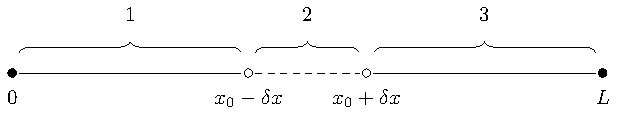
\includegraphics{figures/glitch-1d-example-diagram.pdf}
    \caption[A diagram showing a one-dimensional medium with a small structural perturbation.]{A diagram showing a one-dimensional medium split into three regions. 1: Fixed at \(x=0\) with a constant speed of sound \(c\); 2: A small structural perturbation starting at \(x=x_0\) with width \(\delta x\) with constant speed of sound \(c + \delta c\); 3: Fixed at \(x=L\) with a constant speed of sound \(c\).}
    \label{fig:1d-diagram}
\end{figure}

Initially neglecting the fixed points at \(x = 0, L\), the boundary conditions for this system are,
%
\begin{align}
    \xi_1(x_0, t) &= \xi_2(x_0, t), \\
    \xi_2(x_0 + \delta x) &= \xi_3(x_0 + \delta x), \\
    \frac{\partial \xi_1}{\partial x}(x_0, t) &= \frac{\partial \xi_2}{\partial x}(x_0, t), \\
    \frac{\partial \xi_1}{\partial x}(x_0 + \delta x, t) &= \frac{\partial \xi_2}{\partial x}(x_0 + \delta x, t).
\end{align}
%
Solving these simultaneously gives the following equations for the complex coefficients,
%
\begin{align}
    A &= \delta k (2k + \delta k) (1 - e^{2i \delta x (k + \delta k)}) e^{- 2i k x_0} \alpha^{-1}, \\
    B &= 2 k (2k + \delta_k) e^{2i \delta x (k + \delta k)} e^{i \delta k x_0} \alpha^{-1}, \\
    C &= 2 k \delta k e^{- i x_0 (2k + \delta k)} \alpha^{-1}, \\
    D &= 4 k (k + \delta k) e^{i \delta x (2k + \delta k)} \alpha^{-1},
\end{align}
%
where,
\begin{equation}
    \alpha = (2k + \delta k)^2 e^{2 i \delta x (k + \delta k)} - \delta k^2.
\end{equation}
%

Now we have solutions for the coefficients, we can superpose the right-travelling wave, \(\xi\{k, \delta k\} \rightarrow - \xi\{-k, -\delta k\}\) to get the full solution for the wave function. Substituting \(k, \delta k \rightarrow -k, -\delta k\) into the coefficients yields their complex conjugates. Then, substituting Euler's formula, \(A = (r_A/2) e^{i\phi_A}\), equation \ref{eq:xi1-r} now becomes,
%
\begin{equation}
    \xi_1(x, t) = e^{i \omega t} \left[ \frac{r_A}{2} \left( e^{i(kx + \phi_A)} - e^{-i(kx + \phi_A)} \right) - \left( e^{ikx} - e^{-ikx} \right) \right] \label{eq:xi1}
\end{equation}
%
for which the real solution is,
\begin{equation}
    \real\left[\xi_1(x, t)\right] = \sin \omega t \left[2 \sin kx - r_A \sin(kx + \phi_A)\right]. \label{eq:xi1-real}
\end{equation}
%
However, this does not satisfy the boundary condition that \(\xi_1(0, t) = 0\). To satisfy this, we introduce a small displacement phase \(\epsilon\) and let \(x \rightarrow x + \epsilon\). Solving equation \ref{eq:xi1-real} for \(\epsilon\) at \(x=0\) gives,
%
\begin{align}
    \epsilon &= \frac{1}{k} \tan^{-1}\left( \frac{(r_A / 2) \sin(\phi_A)}{1 - (r_A/2) \cos(\phi_A)} \right), \\
    &= \frac{1}{k} \tan^{-1}\left( \frac{\imag[A]}{1 - \real[A]} \right)
\end{align}
%

We may now write solutions to the wave function in each region. Superposing the right-travelling wave and substituting Euler's formula in a similar way to \ref{eq:xi1} for Equations \ref{eq:xi2-r} and \ref{eq:xi3-r}, we can write the real components of the displacement in each region as,
%
% \begin{align}
%     \xi_3(x, t) = \frac{r_A}{2} e^{i \omega t} \left[ e^{i(k(x + \epsilon) + \phi_A)} - e^{-i(k(x + \epsilon) + \phi_A)} \right],
% \end{align}
%
% with a real solution in trigonometric form,
%
\begin{align}
    \real[\xi_1(x, t)] &= \sin \omega t \left\{2 \sin[k (x + \epsilon)] - r_A \sin[k(x + \epsilon) - \phi_A]\right\} \\
    \real[\xi_2(x, t)] &= \sin \omega t \left\{ r_B \sin[(k + \delta k)(x + \epsilon) - \phi_B] - r_C \sin[(k + \delta k)(x + \epsilon) - \phi_C]\right\} \\
    \real[\xi_3(x, t)] &= \sin \omega t \left\{r_D \sin[k(x + \epsilon) - \phi_D]\right\}
\end{align}
%

Finally, we must impose the boundary condition \(\xi_3(L, t) = 0\) to solve for \(\omega\).
%
\begin{align}
    \sin \omega t \left\{r_D \sin[k(L + \epsilon) - \phi_D]\right\} &= 0, \quad (\div \sin \omega t)\\
    r_D \cos \phi_D \sin[k(L + \epsilon)] - r_D \sin \phi_D \cos[k(L + \epsilon)] &= 0,\\
    \real[D] \sin[k(L + \epsilon)] - \imag[D] \cos[k(L + \epsilon)] &=0. \label{eq:1d-glitch-sol}
\end{align}
%
Solving equation \ref{eq:1d-glitch-sol} for \(\omega\) is not possible analytically. However, we can find individual modes \(\omega_n\) numerically, using equation \ref{eq:omega-n} as initial guesses.

We find the roots \(\omega_n\) of equation \ref{eq:1d-glitch-sol} using Newton's method for \(n = 1,\dots,50\) with \(c=1\), \(L=1\), and several values of \(x_0, \delta x, \delta c\). The difference between the solutions for \(\omega_n\) and those from a linear medium (equation \ref{eq:omega-n}) are shown in Figure \ref{fig:1d-results}. We can see that the change in frequency, \(\delta \omega\) induced by the glitch oscillates. As the location of the glitch, \(x_0\) moves towards the center of the system, \(\delta\omega\) oscillates at a higher frequency. Increasing the width of the glitch, \(\delta x\), modulates the amplitude of \(\delta\omega\), and increasing \(\delta c\) increases the amplitude of \(\delta\omega\).

\begin{figure}
    \centering
    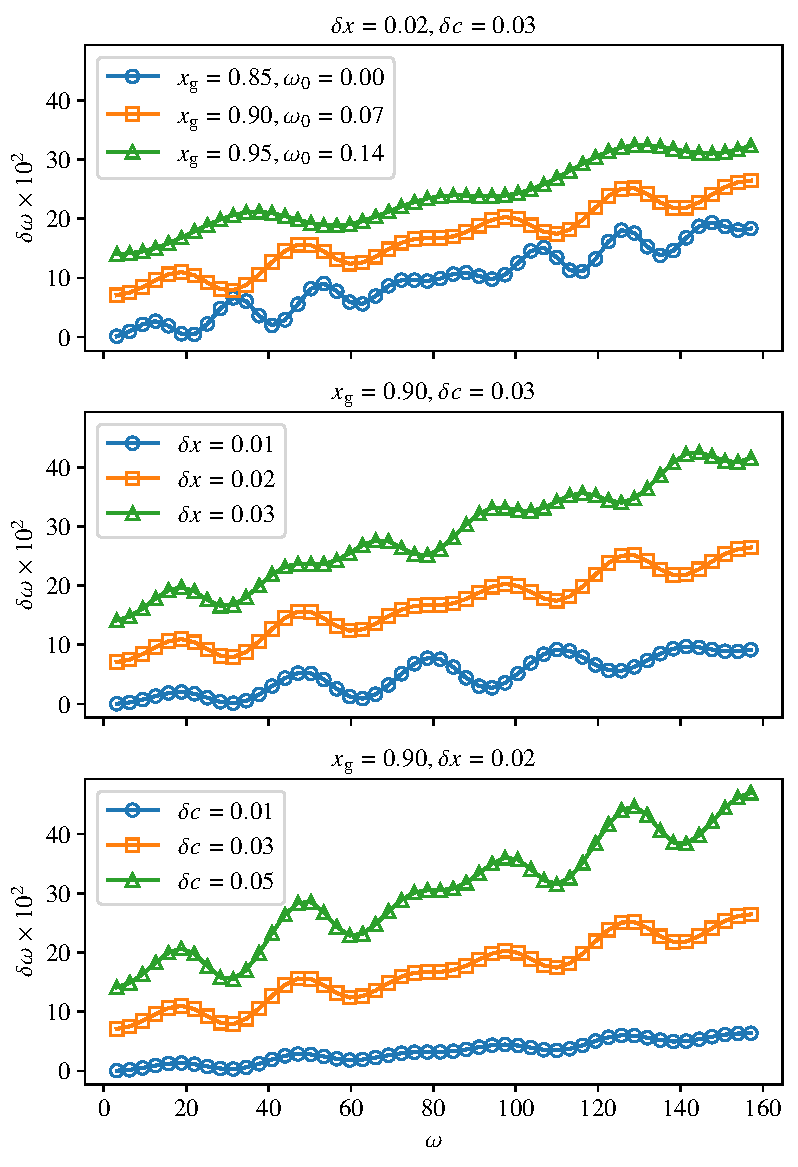
\includegraphics{figures/glitch-1d-example-results.pdf}
    \caption{The change in mode frequency induced by a change in sound speed of \(\delta c\) from \(x=x_0\) to \(x=x_0 + \delta x\) in a one-dimensional medium, bound such that \(x \in [0, 1]\) (see Figure \ref{fig:1d-diagram}). Outside of the perturbation the speed of sound, \(c=1\).
    % The frequencies in the each panel are offset by \(\omega_0\), given in the legend of the top panel.
    }
    \label{fig:1d-results}
\end{figure}

%This may be interpreted as the nodes of each standing wave passing in and out of region 2 with increasing \(n\). Where there is a node, the wave is least sensitive to a change in structure, and 

Now write some stuff about the phase offset \(epsilon\).

\begin{figure}
    \centering
    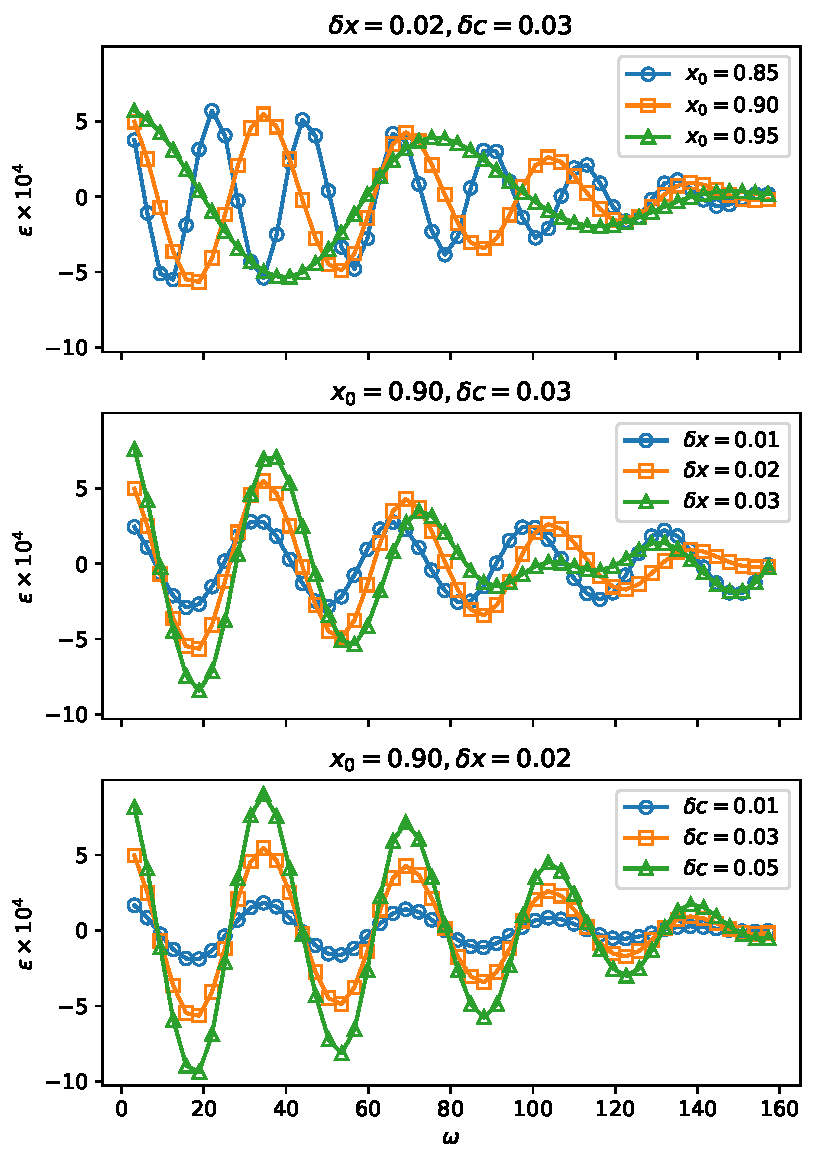
\includegraphics{figures/glitch-1d-example-phase.pdf}
    \caption{The same as Figure \ref{fig:1d-results} but showing the phase offset \(\epsilon\) required to satisfy the boundary conditions.}
    \label{fig:1d-phase}
\end{figure}


It would not be hard to believe that a similar oscillation could be found in the mode frequencies of a star, although its structure is more complicated. We can see from Figure \ref{fig:1d-results} that measuring \(\delta\omega\) could help characterise the structural glitch.

\subsection{Helium glitch}\label{sec:helium-glitch}

Where does the helium glitch come from?

How Tassoul's asymptotic approximation assumes adiabatic exponent of 5/3 but this is not correct for a star. In a star, gamma is effected by the ionisation of elements. This effects the speed of sound,

\begin{equation}
    c = \sqrt{\gamma \frac{p}{\rho}},
\end{equation}

where \(p\) is pressure, \(\rho\) is density, and \(\gamma\) is the first adiabatic exponent,

\begin{equation}
    \gamma \equiv \Gamma_1 = \left( \frac{\partial \ln p}{\partial \ln \rho} \right)_s,
\end{equation}

where \(s\) is specific entropy.

We can simplify the problem to consider a star of just hydrogen and helium. Using the approach of Houdeyer we can derive an apporximation for \(\gamma\) in terms of temperature and density in the star

Reference Houdeyer's paper with plots to show the depression in the first adiabatic exponent with temperature and pressure. 

\begin{figure}
    \centering
    \includegraphics{example-image-a}
    \caption{Multi-panel figure showing \(\gamma\) as a function of \(\rho\) and \(T\) for different values of helium abundance.}
    \label{fig:gamma-temp-density}
\end{figure}

Now we look at the radial order kernels and how they are sensitive to different region


One approach is in Houdek and Gough, to take a perturbation in gamma and propagate this to a perturbation in frequency.

\subsection{Base of the convective zone glitch}\label{sec:bcz-glitch}

Other glitches are present. Sharp structure variation

\section[Modelling the glitch]{Modelling glitches in stellar oscillations}


\subsection{Gaussian processes }\label{sec:glitch-gp}

